\documentclass[11pt,a4paper]{article}

\usepackage[utf8]{inputenc}
\usepackage[T1]{fontenc}
\usepackage{babel}
\babelprovide[import,main]{spanish}
\usepackage{amsmath,amssymb,amsthm}
\usepackage{physics}
\usepackage{bm}
\usepackage{geometry}
\geometry{margin=2.4cm}
\usepackage{graphicx}
\usepackage{booktabs}
\usepackage{algorithm}
\usepackage{algpseudocode}
\usepackage{xcolor}
\usepackage{mdframed}
\usepackage{enumitem}
\usepackage{listings}
\usepackage[hidelinks,colorlinks=true,linkcolor=blue!55!black,citecolor=teal!60!black,urlcolor=blue!55!black]{hyperref}

% --- Estilo para listados de codigo (Python / C++) ---
\definecolor{codegray}{rgb}{0.5,0.5,0.5}
\definecolor{codegreen}{rgb}{0.0,0.45,0.18}
\definecolor{codeblue}{rgb}{0.10,0.20,0.6}
\definecolor{codered}{rgb}{0.65,0.12,0.12}
\definecolor{codebg}{rgb}{0.975,0.975,0.975}
\lstdefinestyle{qmpe}{
  backgroundcolor=\color{codebg},
  basicstyle=\ttfamily\scriptsize,
  commentstyle=\color{codegreen}\itshape,
  keywordstyle=\color{codeblue}\bfseries,
  stringstyle=\color{codered},
  numberstyle=\tiny\color{codegray},
  numbers=left, numbersep=5pt,
  breaklines=true, breakatwhitespace=false,
  showstringspaces=false, tabsize=2, captionpos=b,
  frame=single, rulecolor=\color{codegray!40},
}
\lstset{style=qmpe}

% --- evita choques de \div / \Re ... del paquete physics con español ---
\theoremstyle{definition}
\newtheorem{definicion}{Definición}[section]
\theoremstyle{plain}
\newtheorem{teorema}{Teorema}[section]
\newtheorem{proposicion}{Proposición}[section]
\newtheorem{observacion}{Observación}[section]

\newcommand{\Lop}{\mathcal{L}}
\newcommand{\Ldual}{\mathcal{L}^{\dagger}}
\newcommand{\Dop}{\mathcal{D}}
\newcommand{\Hs}{\mathcal{H}}
\newcommand{\rss}{\rho_{\mathrm{ss}}}
\renewcommand{\Tr}{\operatorname{Tr}}
\newcommand{\vecop}[1]{\operatorname{vec}\!\left(#1\right)}

\newmdenv[linecolor=teal!55!black,linewidth=0.8pt,backgroundcolor=teal!4,
  roundcorner=4pt,skipabove=8pt,skipbelow=8pt,innertopmargin=6pt,innerbottommargin=6pt]{cajaclave}

\title{\textbf{El efecto Mpemba cuántico:\\ marco teórico, espectral y numérico\\ para una implementación paralela en HPC}}
\author{Informe técnico}
\date{\today}

\begin{document}
\maketitle

\begin{abstract}
\noindent
El \emph{efecto Mpemba} designa la relajación anómala en la que un sistema preparado más lejos del equilibrio
alcanza el estado estacionario antes que uno preparado más cerca. En su versión cuántica (QMpE, \emph{quantum
Mpemba effect}) el fenómeno se formula sobre la dinámica disipativa de sistemas cuánticos abiertos y se
explica, en el régimen markoviano, mediante la estructura espectral del generador de Lindblad (el
Liouvilliano $\Lop$): la anomalía aparece cuando el estado inicial tiene un solapamiento anómalamente
pequeño —o nulo— con los modos de decaimiento lentos. Este informe desarrolla de forma explícita y
autocontenida (i)~el formalismo de la ecuación maestra de Gorini--Kossakowski--Sudarshan--Lindblad (GKSL);
(ii)~la descomposición espectral del Liouvilliano y la condición de no-normalidad que sostiene el efecto;
(iii)~la definición operacional del QMpE mediante distintas funciones de distancia y el criterio de
solapamiento $\Tr(\hat l_2\,\rho_0)=0$; (iv)~las variantes principales (Mpemba fuerte, inverso, aceleración
por rotación unitaria global, asimetría de entrelazamiento/restauración de simetría en sistemas de muchos
cuerpos y la interpretación termométrica como recurso); (v)~los modelos paradigmáticos resolubles; y,
sobre todo, (vi)~la \textbf{formulación numérica orientada a HPC}: vectorización del Liouvilliano,
estructura dispersa, escalado de memoria $d^2\times d^2$, métodos de diagonalización densa frente a métodos
de Krylov/Arnoldi para los modos lentos, acción del exponencial de matriz, integración temporal,
trayectorias cuánticas (\emph{embarrassingly parallel}) y redes tensoriales para muchos cuerpos. Se propone
una arquitectura de software y una estrategia de paralelización (MPI + OpenMP + GPU) junto con un
\emph{pipeline} computacional reproducible para tener dominio cuantitativo del fenómeno. El informe se
acompaña de una \textbf{implementación de referencia} (carpeta \texttt{mpemba-cuantico/}): un núcleo
en Python para el estudio y validación del fenómeno en pocos cuerpos, y un núcleo HPC en C++ (MPI${+}$OpenMP)
con las primitivas paralelizables y las costuras marcadas para escalar a muchos cuerpos.
\end{abstract}

\tableofcontents
\bigskip

%====================================================================
\section{Introducción: del Mpemba clásico al cuántico}
%====================================================================

La observación de que, bajo condiciones idénticas de enfriamiento, una muestra de agua inicialmente más
caliente puede congelarse antes que una más fría fue documentada de forma sistemática por Mpemba y Osborne
a finales de los años sesenta \cite{MpembaOsborne1969}, aunque la idea es mucho más antigua. Durante décadas
el fenómeno fue controvertido y dependiente de detalles experimentales difíciles de controlar
(convección, evaporación, sobreenfriamiento, gases disueltos). El cambio de paradigma llegó al reconocer
que el ``efecto Mpemba'' no es una propiedad del agua, sino una propiedad genérica de la \emph{relajación
fuera del equilibrio}: puede definirse de forma limpia y universal en cualquier sistema cuya dinámica
admita un estado estacionario único y una noción de ``distancia al equilibrio'' \cite{LuRaz2017,KlichRaz2019,Bechhoefer2021,Teza2026}.

Esta reformulación abstracta tuvo dos consecuencias. Primero, permitió demostrar y observar el efecto en
plataformas controladas: fluidos granulares \cite{Lasanta2017,Biswas2020}, coloides en trampas ópticas con
control de \emph{feedback} \cite{KumarBechhoefer2020,Kumar2022}, y vidrios de espín
\cite{BaityJesi2019}. Segundo, abrió la puerta a su análogo cuántico. En un sistema cuántico abierto
markoviano la dinámica del operador densidad $\rho$ está gobernada por un generador lineal $\Lop$ (el
Liouvilliano), cuyo espectro determina las escalas de relajación. El \emph{efecto Mpemba cuántico} (QMpE)
ocurre cuando un estado inicial más alejado del estacionario relaja más rápido porque proyecta poco sobre
los modos lentos de $\Lop$ \cite{Carollo2021,KumarLutz2020,Nava2024,Moroder2024,AresCalabreseMurciano2025}.

El interés del QMpE no es meramente conceptual. Permite \emph{acelerar exponencialmente} la convergencia al
estado estacionario mediante una operación de preparación adecuada \cite{Carollo2021,Kochsiek2022},
lo que es directamente relevante para inicialización de \emph{qubits}, preparación de estados estacionarios
disipativos y optimización de motores cuánticos. Más aún, se ha demostrado teóricamente y observado en
simuladores cuánticos, iones atrapados, puntos cuánticos y circuitos
\cite{Joshi2024,AharonyShapira2024,Zhang2025,Chatterjee2023,Liu2024}, y se ha reinterpretado como un
\emph{recurso} metrológico para termometría cuántica fuera del equilibrio
\cite{Chattopadhyay2026,LiYang2026}. La contrapartida es que la simulación cuantitativa del fenómeno
—especialmente en muchos cuerpos— es costosa: el espacio de operadores escala como $d^2$ con la dimensión
$d$ del espacio de Hilbert, lo que motiva una implementación en HPC.

\paragraph{Objetivo del informe.} Proporcionar el marco teórico y numérico necesario para implementar,
verificar y explotar el QMpE en un entorno de cómputo de alto rendimiento. Se prioriza la explicitud
matemática (todas las cantidades necesarias para programar aparecen escritas) y la conexión directa con
algoritmos paralelizables.

%====================================================================
\section{Dinámica de sistemas cuánticos abiertos markovianos}
%====================================================================

\subsection{La ecuación maestra GKSL}

Consideremos un sistema cuántico con espacio de Hilbert $\Hs$ de dimensión finita $d=\dim\Hs$, descrito por
una matriz densidad $\rho$ (operador semidefinido positivo, hermítico, de traza unidad). Cuando el sistema
está débilmente acoplado a un entorno markoviano sin memoria, su evolución reducida está generada por un
mapa lineal $\Lop$ que admite la forma canónica de
Gorini--Kossakowski--Sudarshan--Lindblad \cite{GKS1976,Lindblad1976,BreuerPetruccione2002}:
\begin{equation}
\dv{\rho}{t} \;=\; \Lop[\rho]
\;=\; -\,i\,[H,\rho] \;+\; \Dop[\rho],
\qquad
\Dop[\rho]=\sum_{\mu=1}^{N_J}\!\left( L_\mu\,\rho\,L_\mu^{\dagger}
-\tfrac12\big\{L_\mu^{\dagger}L_\mu,\,\rho\big\}\right),
\label{eq:gksl}
\end{equation}
con $\hbar=1$. Aquí $H=H^{\dagger}$ es el hamiltoniano (parte coherente) y los \emph{operadores de salto}
$\{L_\mu\}_{\mu=1}^{N_J}$ codifican los canales disipativos inducidos por el entorno. El superoperador
$\Lop$ genera una dinámica \emph{completamente positiva y que preserva la traza} (CPTP), garantizando que
$\rho_t=e^{t\Lop}[\rho_0]$ siga siendo un estado físico para todo $t\ge0$ \cite{Carollo2021}.

Dos propiedades estructurales son inmediatas y centrales para todo lo que sigue:
\begin{align}
\Tr\!\big(\Lop[X]\big) &= 0 \qquad \text{(preservación de la traza)},\\
\big(\Lop[X]\big)^{\dagger} &= \Lop[X^{\dagger}] \qquad \text{(preservación de la hermiticidad)}.
\end{align}

\subsection{El mapa dual (representación de Heisenberg)}

Asociado a $\Lop$ existe un mapa adjunto $\Ldual$ que evoluciona observables en lugar de estados
(imagen de Heisenberg) \cite{Carollo2021,LiYang2026}:
\begin{equation}
\Ldual[O]\;=\;+\,i\,[H,O]\;+\;\sum_{\mu=1}^{N_J}\!\left( L_\mu^{\dagger}\,O\,L_\mu
-\tfrac12\big\{L_\mu^{\dagger}L_\mu,\,O\big\}\right).
\label{eq:dual}
\end{equation}
La relación de dualidad es respecto al producto interno de Hilbert--Schmidt
$\langle A,B\rangle_{\mathrm{HS}}=\Tr(A^{\dagger}B)$, esto es
$\langle O,\Lop[\rho]\rangle_{\mathrm{HS}}=\langle \Ldual[O],\rho\rangle_{\mathrm{HS}}$.
La distinción entre $\Lop$ y $\Ldual$ es esencial: sus autovectores (modos derechos e izquierdos)
\emph{no coinciden}, y es justamente esa asimetría la que da lugar al efecto Mpemba.

%====================================================================
\section{Descomposición espectral del Liouvilliano}
%====================================================================

\subsection{Autovalores y autooperadores}

Suponiendo $\Lop$ diagonalizable, definimos los \emph{autooperadores derechos} $\hat r_k$ y los
\emph{autooperadores izquierdos} $\hat l_k$ mediante \cite{Carollo2021,LiYang2026}:
\begin{equation}
\Lop[\hat r_k]=\lambda_k\,\hat r_k,
\qquad
\Ldual[\hat l_k]=\lambda_k^{*}\,\hat l_k,
\qquad k=1,\dots,d^2 .
\label{eq:eig}
\end{equation}
Los autovalores $\lambda_k\in\mathbb{C}$ del Liouvilliano cumplen propiedades dictadas por la estructura
CPTP \cite{Carollo2021,Minganti2018}:
\begin{enumerate}[leftmargin=1.6em,itemsep=2pt]
\item $\operatorname{Re}(\lambda_k)\le 0$ para todo $k$ (estabilidad; los modos decaen, no crecen).
\item Si $\lambda_k$ es complejo, su conjugado $\lambda_k^{*}$ también es autovalor (preservación de la
hermiticidad); si $\lambda_k$ es real, $\hat r_k$ puede elegirse hermítico.
\item Existe al menos un autovalor nulo $\lambda_1=0$. Si es no degenerado, el \textbf{estado
estacionario} es único:
\begin{equation}
\rss=\lim_{t\to\infty}\rho_t=\hat r_1,\qquad \Tr(\hat r_1)=1,\qquad \hat l_1=\mathbb{1}.
\end{equation}
\end{enumerate}
Las bases derecha e izquierda pueden normalizarse para ser \emph{biortonormales}:
\begin{equation}
\Tr\!\big(\hat l_j^{\dagger}\,\hat r_k\big)=\delta_{jk}.
\label{eq:biorth}
\end{equation}

\subsection{Dinámica como suma de modos}

Con la base biortonormal, la evolución de cualquier estado inicial $\rho_0$ admite la representación
espectral exacta \cite{Carollo2021,LiYang2026,Chattopadhyay2026}:
\begin{equation}
\boxed{\;
\rho_t=e^{t\Lop}[\rho_0]
=\rss+\sum_{k=2}^{d^2}\, e^{\lambda_k t}\,
\underbrace{\Tr\!\big(\hat l_k^{\dagger}\rho_0\big)}_{\displaystyle a_k\ \text{(solapamiento inicial)}}\,
\hat r_k \;}
\label{eq:spectral}
\end{equation}
Cada $\hat r_k$ ($k\ge2$) es un \emph{modo de excitación} que decae con tasa $|\!\operatorname{Re}(\lambda_k)|$.
Ordenamos los autovalores por parte real creciente en módulo,
\begin{equation}
0=|\operatorname{Re}(\lambda_1)| < |\operatorname{Re}(\lambda_2)| \le |\operatorname{Re}(\lambda_3)| \le\cdots,
\end{equation}
de modo que, a tiempos largos, la relajación está dominada por el \textbf{modo más lento} $\hat r_2$
(suponiendo $\lambda_2$ real y único). La escala de relajación global es
\begin{equation}
\tau=\frac{1}{|\operatorname{Re}(\lambda_2)|}.
\label{eq:tau}
\end{equation}

\subsection{No-normalidad: el corazón del efecto Mpemba}

El Liouvilliano es genéricamente \emph{no normal}: $\Lop\,\Ldual\neq\Ldual\,\Lop$. Como consecuencia, los
autooperadores derechos \emph{no son ortogonales} entre sí, $\Tr(\hat r_i^{\dagger}\hat r_j)\neq0$ para
$i\neq j$ \cite{LiYang2026,Minganti2018}. Esta no-normalidad implica que:
\begin{itemize}[leftmargin=1.6em,itemsep=2pt]
\item Los coeficientes $a_k=\Tr(\hat l_k^{\dagger}\rho_0)$ dependen de \emph{autovectores izquierdos}, que
difieren de los derechos. Un estado puede estar ``lejos'' del equilibrio (gran norma de la desviación
$\rho_0-\rss$) y, sin embargo, tener $a_2\approx0$.
\item Pueden aparecer transitorios no monótonos y crecimientos transitorios de la distancia
(\emph{transient amplification}) antes del decaimiento, fenómeno típico de operadores no normales.
\end{itemize}

\begin{cajaclave}
\textbf{Idea física central.} El efecto Mpemba cuántico no es una violación de la termodinámica: es una
consecuencia de la geometría \emph{no ortogonal} de los modos de relajación. Un estado preparado para
solapar poco con el modo lento $\hat r_2$ ``salta'' la escala temporal $\tau$ y relaja gobernado por modos
más rápidos, adelantando a estados aparentemente más cercanos al equilibrio.
\end{cajaclave}

%====================================================================
\section{Definición operacional del efecto Mpemba cuántico}
%====================================================================

\subsection{Funciones de distancia al equilibrio}

Para hablar de ``más cerca'' o ``más lejos'' del estacionario hace falta una función de distancia
$\Dop(\rho_t\|\rss)$, monótonamente decreciente bajo mapas CPTP. Las elecciones habituales son
\cite{KumarBechhoefer2020,LiYang2026,Alyuruk2025}:
\begin{align}
\text{Distancia de traza:}\quad & D_{\mathrm{tr}}(\rho\|\rss)=\tfrac12\,\norm{\rho-\rss}_1
=\tfrac12\,\Tr\sqrt{(\rho-\rss)^{\dagger}(\rho-\rss)},\\[2pt]
\text{Norma de Hilbert--Schmidt:}\quad & D_{\mathrm{HS}}(\rho\|\rss)=\norm{\rho-\rss}_2
=\sqrt{\Tr\!\big[(\rho-\rss)^2\big]},\\[2pt]
\text{Divergencia de Kullback--Leibler:}\quad & D_{\mathrm{KL}}(p\|\pi)=\sum_i p_i\,\ln\!\frac{p_i}{\pi_i},\\[2pt]
\text{Entropía relativa cuántica:}\quad & S(\rho\|\rss)=\Tr\!\big[\rho(\ln\rho-\ln\rss)\big].
\end{align}
Para estados diagonales en la base de energía, $\rho$ se reduce a un vector de poblaciones $p_i$ y la
$D_{\mathrm{KL}}$ se conecta con la energía libre fuera del equilibrio,
$F_{\mathrm{neq}}=F_{\mathrm{eq}}+k_BT\,D_{\mathrm{KL}}(p\|\pi)$
\cite{KumarBechhoefer2020}. Es importante que la \emph{existencia} del cruce de curvas (la firma del
efecto) es robusta frente a la elección de distancia, aunque los detalles cuantitativos cambien
\cite{KumarBechhoefer2020}.

\subsection{El criterio del cruce y del solapamiento}

\begin{definicion}[Efecto Mpemba cuántico]
Sean dos preparaciones $\rho^{\mathrm{cal}}_0$ (``caliente'', más lejos) y $\rho^{\mathrm{fr}}_0$
(``fría'', más cerca), con
$\Dop(\rho^{\mathrm{cal}}_0\|\rss) > \Dop(\rho^{\mathrm{fr}}_0\|\rss)$.
Hay efecto Mpemba si existe un tiempo de cruce $t^{*}$ tal que
\begin{equation}
\Dop\!\big(\rho^{\mathrm{cal}}_{t}\,\|\,\rss\big) \;<\; \Dop\!\big(\rho^{\mathrm{fr}}_{t}\,\|\,\rss\big)
\qquad \forall\, t> t^{*}.
\end{equation}
\end{definicion}

A partir de la ecuación \eqref{eq:spectral}, a tiempos suficientemente largos
$\Dop(\rho_t\|\rss)\sim |a_2|\,e^{-|\operatorname{Re}\lambda_2| t}\,\norm{\hat r_2}$. El estado que termina
más cerca es el que tiene \emph{menor} coeficiente $|a_2|$ sobre el modo lento. El caso extremo es:

\begin{cajaclave}
\textbf{Criterio de solapamiento (Mpemba fuerte / \emph{strong}).} Si la preparación caliente se diseña de
modo que su proyección sobre el modo izquierdo lento se anule,
\begin{equation}
a_2=\Tr\!\big(\hat l_2^{\dagger}\,\rho^{\mathrm{cal}}_0\big)=0,
\label{eq:strong}
\end{equation}
entonces el término $e^{\lambda_2 t}$ desaparece de \eqref{eq:spectral} y la relajación pasa a estar
gobernada por $\lambda_3$ (o el siguiente modo con solapamiento no nulo). La convergencia se
\textbf{acelera exponencialmente}, con un nuevo tiempo $\tau'=1/|\operatorname{Re}\lambda_3|<\tau$
\cite{Carollo2021,Zhang2025}.
\end{cajaclave}

\noindent
El criterio \eqref{eq:strong} es \emph{conveniente} pero, en rigor, \emph{ni necesario ni suficiente} para
el cruce de distancias: el efecto puede ocurrir con solapamiento no nulo sobre todos los modos, por
combinación de signos y normas de los $\hat r_k$ \cite{LiYang2026}. En la práctica numérica conviene medir
directamente la distancia $\Dop(\rho_t\|\rss)$ \emph{y}, como diagnóstico, los solapamientos
$a_k$.

%====================================================================
\section{Mecanismos, variantes y conexiones físicas}
%====================================================================

\subsection{Aceleración exponencial por rotación unitaria global (Carollo--Lasanta--Lesanovsky)}

Una aplicación operacional notable consiste en aplicar, justo antes de la dinámica disipativa, una
transformación unitaria $U$ que lleve el estado inicial a un subespacio que no excite el modo lento
\cite{Carollo2021,Kochsiek2022}. Formalmente, se busca $U$ tal que
\begin{equation}
\Tr\!\big(\hat l_2^{\dagger}\,U\rho_0 U^{\dagger}\big)=0,
\end{equation}
con lo que se evitan regímenes metaestables de larga duración. Esto se demostró explícitamente en modelos
de Dicke y en sistemas de espín con interacción ``todos con todos'', logrando aceleraciones exponenciales
de la aproximación a la estacionariedad \cite{Carollo2021}. En sistemas de muchos cuerpos basta a menudo una
rotación de espín \emph{global} (un único parámetro), lo que la hace experimentalmente viable
\cite{Kochsiek2022}.

\subsection{Efecto Mpemba inverso}

El fenómeno simétrico también existe: un sistema inicialmente más \emph{frío} puede \emph{calentarse} más
rápido que uno más caliente cuando ambos se ponen en contacto con un baño caliente
\cite{LuRaz2017,AharonyShapira2024}. La condición suficiente, en el lenguaje espectral, intercambia el papel
de las preparaciones y exige que la preparación fría solape poco con el modo lento. El efecto inverso se ha
demostrado experimentalmente en un \emph{qubit} de ion atrapado con disipación diseñada
\cite{AharonyShapira2024}.

\subsection{Mpemba múltiple, puntos excepcionales y oscilaciones}

Cuando $\lambda_2$ es complejo (modos con parte imaginaria) la relajación incorpora oscilaciones
amortiguadas, y pueden producirse \emph{múltiples cruces} de las curvas de distancia. La coalescencia de
autovalores y autovectores del Liouvilliano en \emph{puntos excepcionales} (no diagonalizabilidad,
bloques de Jordan) genera dependencias temporales polinomiales $t^{n}e^{\lambda t}$ y enriquece la
fenomenología \cite{Chatterjee2024,Minganti2018}. Numéricamente esto obliga a manejar la posibilidad de que
$\Lop$ no sea diagonalizable (forma de Schur/Jordan).

\subsection{Asimetría de entrelazamiento y restauración de simetría (muchos cuerpos)}

En sistemas cerrados de muchos cuerpos surge una versión distinta del QMpE asociada a la \emph{restauración
dinámica de una simetría} tras un \emph{quench} \cite{AresCalabreseMurciano2025,Murciano2024,Rylands2024,Liu2024,Joshi2024}.
La cantidad relevante es la \emph{asimetría de entrelazamiento} $\Delta S_A$, que mide cuánto rompe el estado
reducido de un subsistema $A$ una simetría dada (por ejemplo, $U(1)$ de conservación del número de
partículas). El efecto Mpemba aparece cuando un estado inicial que rompe \emph{más} la simetría la
restaura \emph{antes}. Esta línea condujo a la primera observación experimental del QMpE en un simulador de
iones atrapados \cite{Joshi2024} y a una comprensión microscópica en sistemas integrables vía la imagen de
cuasipartículas \cite{Rylands2024}. Para HPC, esta variante exige métodos de \emph{redes tensoriales}
(MPS/TEBD) más que diagonalización del Liouvilliano, por el escalado del espacio de Hilbert.

\subsection{Del anómalo al recurso: termometría cuántica}

Recientemente el QMpE se ha reinterpretado como un \emph{recurso} metrológico. La idea: la sensibilidad de
una sonda a la temperatura del baño se cuantifica con la \emph{información cuántica de Fisher} (QFI)
$F_T[\rho_t]$, ligada a la cota de Cramér--Rao $\Delta T^2 \ge 1/F_T[\rho]$ \cite{Chattopadhyay2026,LiYang2026}.
Para un estado diagonal en la base de energía con poblaciones $p_i(t)$,
\begin{equation}
F_T[\rho_t]=\sum_i \frac{\big(\partial_T p_i(t)\big)^2}{p_i(t)} .
\label{eq:qfi}
\end{equation}
El resultado central es que toda \emph{inversión de Mpemba} en la relajación produce un aumento de
\emph{tiempo finito} de la QFI: las preparaciones calientes fuera del equilibrio pueden superar
transitoriamente tanto a las preparaciones frías como a la estrategia de equilibrio
\cite{Chattopadhyay2026,LiYang2026}. Esto convierte la relajación anómala en una herramienta de termometría
ultrarrápida a nanoescala, y motiva mapear computacionalmente el ``paisaje'' de QFI a lo largo de la
relajación.

\subsection{Marco unificador de teoría de recursos}

Un desarrollo reciente unifica las variantes clásicas y cuánticas del efecto Mpemba en el lenguaje de las
\emph{teorías de recursos} (termo-mayorización, atermalidad), identificando qué papel juegan las
correlaciones y la coherencia cuántica como ingredientes que pueden ampliar la ``ventana de Mpemba''
\cite{Alyuruk2025,Summer2026}. Para nuestros fines, esto proporciona criterios independientes de la dinámica
(monótonas de recurso) útiles para validar resultados numéricos.

%====================================================================
\section{Modelos paradigmáticos resolubles}
%====================================================================

Antes de escalar a muchos cuerpos conviene fijar bancos de prueba con solución analítica para
\emph{verificar} el código de HPC.

\subsection{Qubit con amortiguamiento de amplitud generalizado (TLS)}

Un sistema de dos niveles (TLS) con separación energética $\omega_0$, acoplado débilmente a un baño bosónico
a temperatura $T$, obedece \cite{Chattopadhyay2026,LiYang2026}:
\begin{equation}
\dv{\rho}{t}=\gamma(\bar n+1)\,\Dop[\sigma_-]\rho+\gamma\,\bar n\,\Dop[\sigma_+]\rho,
\qquad
\bar n(T)=\frac{1}{e^{\omega_0/T}-1},
\label{eq:tls}
\end{equation}
con $\sigma_-=\dyad{0}{1}$, $\sigma_+=\dyad{1}{0}$ y $\Dop[L]\rho=L\rho L^{\dagger}-\tfrac12\{L^{\dagger}L,\rho\}$.
Para un estado inicial diagonal $\rho(0)=\operatorname{diag}(1-p_0,\,p_0)$ la coherencia permanece nula y la
población del estado excitado satisface la ecuación lineal
\begin{equation}
\dv{p}{t}=-\Gamma(T)\,\big[p(t)-p_{\mathrm{eq}}(T)\big],\quad
\Gamma(T)=\gamma\,(2\bar n+1),\quad
p_{\mathrm{eq}}=\frac{\bar n}{2\bar n+1}=\frac{1}{1+e^{\omega_0/T}},
\end{equation}
con solución exacta $p(t)=p_{\mathrm{eq}}+(p_0-p_{\mathrm{eq}})e^{-\Gamma t}$. El TLS de un solo modo es
demasiado simple para mostrar el cruce (relajación monótona con tasa única); el efecto requiere
\emph{múltiples} canales/modos con tasas distintas, como en sistemas $\Lambda$ de tres niveles, dos qubits
acoplados o muchos cuerpos \cite{LiYang2026,Chattopadhyay2026}. Este modelo sirve, por tanto, como prueba de
correctitud del integrador y del cálculo de QFI \eqref{eq:qfi}.

\subsection{Modelo de Dicke y espín colectivo}

El modelo de Dicke (un conjunto de $N$ espines $1/2$ acoplados colectivamente a un modo) admite reducción al
sector totalmente simétrico de dimensión $N+1$, lo que permite explorar el QMpE y la aceleración por
rotación unitaria en sistemas grandes con coste polinómico en $N$ \cite{Carollo2021}. Es el banco de prueba
ideal para validar la estrategia de ``rotación óptima'' antes de pasar al régimen no colectivo.

\subsection{Cadena de espines / Ising disipativo}

La cadena de Ising de $N$ espines con campo transverso y disipación local es el modelo de referencia para el
régimen de muchos cuerpos. El número de microestados crece como $2^N$ y el Liouvilliano vive en un espacio
de dimensión $4^N$, lo que hace de este el caso que \emph{exige} HPC. En la versión estocástica clásica
(dinámica de Glauber/Metropolis con tasas $R_{ij}\propto e^{-(E_i-E_j)/2k_BT}$ para un único \emph{spin
flip}) el efecto ya aparece y conecta con el paisaje energético \cite{LuRaz2017,KlichRaz2019}.

%====================================================================
\section{Formulación numérica para HPC}
%====================================================================

Esta sección traduce el formalismo anterior en objetos computables y discute el coste y la paralelización.

\subsection{Vectorización del Liouvilliano (superoperador matricial)}

El paso clave es convertir la ecuación \emph{de operadores} \eqref{eq:gksl} en una ecuación \emph{de
vectores}. Apilando las columnas de $\rho$ (convención \emph{column-stacking}) se define
$\ket{\rho}\!\rangle=\vecop{\rho}\in\mathbb{C}^{d^2}$. Usando la identidad
$\vecop{A X B}=(B^{\mathsf{T}}\otimes A)\,\vecop{X}$, el generador \eqref{eq:gksl} se representa por una
\textbf{matriz} $\mathbb{L}\in\mathbb{C}^{d^2\times d^2}$ \cite{Minganti2018,Weimer2021}:
\begin{equation}
\boxed{\;
\mathbb{L}= -\,i\big(\mathbb{1}\otimes H - H^{\mathsf{T}}\otimes\mathbb{1}\big)
+\sum_{\mu}\Big[
L_\mu^{*}\otimes L_\mu
-\tfrac12\big(\mathbb{1}\otimes L_\mu^{\dagger}L_\mu
+ (L_\mu^{\mathsf{T}}L_\mu^{*})\otimes\mathbb{1}\big)\Big]\;}
\label{eq:vecL}
\end{equation}
de modo que la dinámica se reduce a un sistema lineal de ecuaciones diferenciales ordinarias
\begin{equation}
\dv{t}\ket{\rho}\!\rangle=\mathbb{L}\,\ket{\rho}\!\rangle,
\qquad
\ket{\rho_t}\!\rangle=e^{t\mathbb{L}}\,\ket{\rho_0}\!\rangle .
\end{equation}
El espectro de $\mathbb{L}$ es exactamente el de $\Lop$; los autovectores de $\mathbb{L}$ son los
$\vecop{\hat r_k}$ (derecha) y los $\vecop{\hat l_k}$ (izquierda, vía $\mathbb{L}^{\dagger}$).

\begin{observacion}[Escalado y memoria]
La dimensión del problema espectral es $d^2$. Para $N$ qubits, $d=2^N$ y $\mathbb{L}$ es $4^N\times4^N$.
Almacenar $\mathbb{L}$ \emph{densa} cuesta $\mathcal{O}(16^N)$ números complejos: inviable más allá de
$N\!\approx\!6$--$7$ en un solo nodo. La diagonalización densa cuesta $\mathcal{O}(d^6)=\mathcal{O}(64^N)$.
Esto fuerza el uso de representaciones \emph{dispersas} y métodos iterativos.
\end{observacion}

\subsection{Estructura dispersa y operaciones fundamentales}

$H$ y los $L_\mu$ de modelos físicos (locales, con interacción a vecinos) son altamente dispersos. Los
productos de Kronecker en \eqref{eq:vecL} preservan la dispersión: $\mathbb{L}$ tiene
$\mathcal{O}(d^2\,\mathrm{poly}(N))$ elementos no nulos. La operación primitiva de todos los métodos
iterativos es el producto \emph{matriz dispersa--vector} (SpMV) $\ket{v}\!\rangle\mapsto\mathbb{L}\ket{v}\!\rangle$,
que conviene implementar \emph{sin materializar} $\mathbb{L}$ (\emph{matrix-free}) aplicando
\eqref{eq:gksl} directamente al operador $V=\operatorname{vec}^{-1}(\ket{v}\!\rangle)$:
\begin{equation}
\mathbb{L}\ket{v}\!\rangle=\vecop{\,-i[H,V]+\textstyle\sum_\mu(L_\mu V L_\mu^{\dagger}-\tfrac12\{L_\mu^{\dagger}L_\mu,V\})}.
\end{equation}
La versión \emph{matrix-free} reduce memoria de $\mathcal{O}(\mathrm{nnz}(\mathbb{L}))$ a
$\mathcal{O}(\mathrm{nnz}(H)+\sum_\mu\mathrm{nnz}(L_\mu))$ y es la base de la escalabilidad.

\subsection{Tres tareas de cómputo y sus algoritmos}

El estudio cuantitativo del QMpE se descompone en tres tareas, con algoritmos y costes distintos.

\paragraph{(T1) Espectro y modos lentos.}
Para diagnosticar el efecto (calcular $\lambda_2,\lambda_3$, los modos $\hat r_2,\hat l_2$ y los
solapamientos $a_k$) \emph{no} hace falta todo el espectro: bastan los pocos autovalores con parte real más
próxima a cero. Es un problema de autovalores \emph{interior} (\emph{eigenvalues closest to a target},
\emph{target} $=0$). El método de elección es \textbf{Arnoldi con reinicio implícito}
(\textsc{arpack}) o, en paralelo, \textsc{slepc} sobre \textsc{petsc}, usando una transformación
\emph{shift-invert} $(\mathbb{L}-\sigma\mathbb{1})^{-1}$ para converger a los modos de interés
\cite{Lehoucq1998,Hernandez2005,Balay2023,Minganti2018}. Coste por iteración: dominado por SpMV (o por una
resolución lineal dispersa si se usa \emph{shift-invert}).

\paragraph{(T2) Evolución temporal.}
Para trazar las curvas de distancia $\Dop(\rho_t\|\rss)$ hay dos vías:
\begin{itemize}[leftmargin=1.6em,itemsep=2pt]
\item \emph{Acción del exponencial}: calcular $\ket{\rho_t}\!\rangle=e^{t\mathbb{L}}\ket{\rho_0}\!\rangle$
sin formar $e^{t\mathbb{L}}$, mediante subespacios de Krylov (\textsc{Expokit}) o el algoritmo de
escalado-y-cuadrado de la acción \cite{Sidje1998,AlMohyHigham2011}. Ideal para muestrear muchos
tiempos a partir del mismo $\rho_0$.
\item \emph{Integración directa}: integradores ODE rígidos de paso adaptativo (BDF, \emph{Runge--Kutta}
implícito) o integradores exponenciales/Magnus para sistemas con dependencia temporal.
\end{itemize}

\paragraph{(T3) Régimen de muchos cuerpos.}
Cuando $4^N$ excede la memoria disponible, se abandona el Liouvilliano explícito y se recurre a:
\begin{itemize}[leftmargin=1.6em,itemsep=2pt]
\item \textbf{Trayectorias cuánticas} (\emph{Monte Carlo wavefunction} / \emph{quantum jumps}): se promedian
$M$ realizaciones estocásticas de vectores de estado $\ket{\psi}\in\mathbb{C}^{d}$ (no operadores
$\in\mathbb{C}^{d^2}$), recuperando $\rho_t=\mathbb{E}[\dyad{\psi_t}{\psi_t}]$ \cite{Daley2014}. Reduce la
memoria de $d^2$ a $d$ y es \textbf{trivialmente paralelizable} (\emph{embarrassingly parallel}): cada
trayectoria es independiente. El error estadístico decae como $M^{-1/2}$.
\item \textbf{Redes tensoriales} para estados mixtos: MPO/MPDO con TEBD disipativo o métodos variacionales,
con coste controlado por la dimensión de enlace $\chi$ \cite{Orus2014,Weimer2021}. Imprescindible para
la variante de asimetría de entrelazamiento en cadenas largas \cite{AresCalabreseMurciano2025}.
\end{itemize}

\subsection{Resumen de costes}

\begin{table}[h]
\centering
\small
\begin{tabular}{@{}llll@{}}
\toprule
Tarea & Método & Coste tiempo (orden) & Memoria (orden) \\
\midrule
Espectro completo & Diagonalización densa & $d^6$ & $d^4$ \\
Modos lentos (T1) & Arnoldi / SLEPc (shift-invert) & $n_{\mathrm{it}}\cdot$SpMV & $\mathrm{nnz}(\mathbb{L})$ \\
Evolución (T2) & Acción de Krylov ($e^{t\mathbb{L}}v$) & $n_{\mathrm{step}}\cdot m\cdot$SpMV & $m\,d^2$ \\
Muchos cuerpos (T3a) & Trayectorias cuánticas & $M\cdot n_{\mathrm{step}}\cdot$SpMV$_d$ & $d$ por trayectoria \\
Muchos cuerpos (T3b) & MPO/TEBD disipativo & $\sim N\chi^3 d_{\mathrm{loc}}^{?}$ & $N\chi^2$ \\
\bottomrule
\end{tabular}
\caption{Comparativa de coste. $d=\dim\Hs$; $m$ = dimensión del subespacio de Krylov; $M$ = número de
trayectorias; $\chi$ = dimensión de enlace. SpMV denota el producto matriz dispersa--vector dominante.}
\end{table}

%====================================================================
\section{Estrategia de paralelización}
%====================================================================

\subsection{Tres niveles de paralelismo}

\begin{enumerate}[leftmargin=1.6em,itemsep=3pt]
\item \textbf{Paralelismo de datos (MPI) sobre el vector de estado/operador.} El vector
$\ket{\rho}\!\rangle\in\mathbb{C}^{d^2}$ se distribuye por bloques de filas entre procesos. El SpMV
\emph{matrix-free} requiere comunicación de halo (intercambio de las componentes que cruzan fronteras de
bloque). \textsc{petsc/slepc} proporciona esta distribución y los \emph{solvers} de forma escalable
\cite{Balay2023,Hernandez2005}. Es el camino para las tareas T1 y T2 hasta el límite de memoria agregada.
\item \textbf{Paralelismo de tareas (\emph{embarrassingly parallel}) sobre trayectorias.} Para T3a, las $M$
trayectorias se reparten entre procesos/nodos sin comunicación salvo la reducción final
($\mathbb{E}[\cdot]$). Escalabilidad casi perfecta; el cuello de botella es la generación de números
aleatorios independientes y la reducción \cite{Daley2014}.
\item \textbf{Paralelismo intranodo (OpenMP / GPU).} Cada SpMV y cada producto de Kronecker dispersos se
aceleran con \emph{threads} (OpenMP) o en GPU (cuSPARSE / bibliotecas de productos tensoriales). Para
muchos cuerpos, las contracciones tensoriales (T3b) se benefician enormemente de GEMM en GPU.
\end{enumerate}

\subsection{Mapa de la implementación recomendada}

\begin{itemize}[leftmargin=1.6em,itemsep=2pt]
\item \textbf{Construcción de $\mathbb{L}$}: ensamblar $H$ y $\{L_\mu\}$ como matrices dispersas
distribuidas; evaluar SpMV \emph{matrix-free} vía \eqref{eq:gksl}.
\item \textbf{T1 (modos lentos)}: \textsc{slepc} (\texttt{EPS}) con \emph{spectral transformation}
\texttt{shift-invert} en $\sigma=0$, \emph{solver} lineal disperso paralelo (\textsc{mumps}/\textsc{superlu\_dist}
o iterativo precondicionado).
\item \textbf{T2 (evolución)}: \textsc{slepc} (\texttt{MFN}, \emph{matrix function}) para $e^{t\mathbb{L}}v$, o
integradores de \textsc{petsc} (\texttt{TS}) con métodos rígidos.
\item \textbf{T3a (trayectorias)}: prototipado con QuTiP \cite{Johansson2013}; producción con un
\emph{driver} MPI que reparte semillas y trayectorias, con SpMV en GPU.
\item \textbf{T3b (redes tensoriales)}: ITensor / TeNPy con \emph{backend} GPU para cadenas largas y la
asimetría de entrelazamiento.
\end{itemize}

\subsection{Pseudocódigo del núcleo de diagnóstico}

\begin{algorithm}[h]
\caption{Diagnóstico del QMpE (espectral + curvas de distancia)}
\begin{algorithmic}[1]
\State \textbf{Entrada:} $H$, $\{L_\mu\}$, conjunto de estados iniciales $\{\rho_0^{(s)}\}$, malla temporal $\{t_n\}$
\State Ensamblar SpMV \emph{matrix-free} de $\mathbb{L}$ y de $\mathbb{L}^{\dagger}$ \Comment{ec. \eqref{eq:gksl},\eqref{eq:dual}}
\State $(\lambda_1{=}0,\hat r_1{=}\rss)\gets$ modo estacionario (núcleo de $\mathbb{L}$) \Comment{T1}
\State $\{\lambda_k,\hat r_k\}_{k\le K}\gets$ Arnoldi shift-invert$(\mathbb{L},\sigma{=}0,K)$ \Comment{modos lentos}
\State $\{\hat l_k\}_{k\le K}\gets$ Arnoldi shift-invert$(\mathbb{L}^{\dagger},\sigma{=}0,K)$; biortonormalizar \eqref{eq:biorth}
\For{cada estado inicial $s$}
  \State $a_k^{(s)}\gets \Tr(\hat l_k^{\dagger}\rho_0^{(s)})$ \Comment{solapamientos, diagnóstico de \eqref{eq:strong}}
  \For{cada $t_n$}
    \State $\rho_{t_n}^{(s)}\gets e^{t_n\mathbb{L}}\,\rho_0^{(s)}$ \Comment{acción de Krylov, T2}
    \State $D^{(s)}(t_n)\gets \Dop(\rho_{t_n}^{(s)}\|\rss)$; \; opcional: $F_T[\rho_{t_n}^{(s)}]$ \eqref{eq:qfi}
  \EndFor
\EndFor
\State Detectar cruces $t^{*}$ entre $D^{(s)}(t)$ y $D^{(s')}(t)$ \Comment{firma del efecto}
\State \textbf{Salida:} $\{\lambda_k\}$, $\{a_k^{(s)}\}$, curvas $D^{(s)}(t)$, tiempos de cruce $t^{*}$
\end{algorithmic}
\end{algorithm}

\subsection{Verificación y reproducibilidad}

\begin{itemize}[leftmargin=1.6em,itemsep=2pt]
\item \textbf{Pruebas de correctitud}: comparar el TLS \eqref{eq:tls} y el modelo de Dicke contra solución
analítica; comprobar $\Tr(\rho_t)=1$ y positividad a lo largo de la evolución.
\item \textbf{Convergencia}: en trayectorias, verificar el escalado $M^{-1/2}$ del error; en Krylov,
verificar independencia respecto a $m$; en redes tensoriales, convergencia en $\chi$.
\item \textbf{Validación física}: contrastar las predicciones con monótonas de recurso
(termo-mayorización) que no dependen del integrador \cite{Alyuruk2025,Summer2026}.
\item \textbf{Trazabilidad}: fijar semillas, registrar versiones de bibliotecas (PETSc/SLEPc, QuTiP) y
exportar espectros y curvas en formato reproducible.
\end{itemize}

%====================================================================
\section{Pipeline computacional propuesto}
%====================================================================

\begin{enumerate}[leftmargin=1.6em,itemsep=3pt]
\item \textbf{Capa de modelo}: definición declarativa de $H(\{J,h,\dots\})$, $\{L_\mu(\gamma,T,\dots)\}$ y
familias de estados iniciales $\rho_0^{(s)}(T_{\mathrm{cal}},T_{\mathrm{fr}})$.
\item \textbf{Capa de ensamblaje}: construcción \emph{matrix-free} de SpMV de $\mathbb{L},\mathbb{L}^{\dagger}$;
distribución MPI del vector $\ket{\rho}\!\rangle$.
\item \textbf{Capa de cálculo}: T1 (SLEPc), T2 (acción de Krylov), T3 (trayectorias / redes tensoriales),
con selección automática según $N$ y memoria disponible.
\item \textbf{Capa de análisis}: distancias, QFI, detección de cruces, búsqueda de la rotación unitaria
óptima $U$ que anula $a_2$ (problema de optimización sobre un grupo de Lie).
\item \textbf{Capa de barrido}: exploración paramétrica masiva (temperaturas, acoplamientos, tamaños $N$)
mediante un planificador de trabajos (SLURM) que aprovecha el paralelismo de tareas.
\end{enumerate}

%====================================================================
\section{Implementación de referencia: validación y resultados}
%====================================================================

Las secciones anteriores fijan el marco teórico y la estrategia de cómputo. Esta
sección documenta la \textbf{capa computacional concreta} que materializa ese
marco y que se distribuye junto a este informe en la carpeta
\texttt{mpemba-cuantico/}. La implementación tiene dos componentes
complementarios:
\begin{enumerate}[leftmargin=1.6em,itemsep=2pt]
\item Una \textbf{implementación de referencia en Python} (\texttt{python/}, solo
\texttt{numpy}) pensada para \emph{estudiar} el fenómeno en pocos cuerpos y servir
de especificación verificable. Implementa la vectorización del Liouvilliano, la
descomposición espectral, la evolución (exacta por modos y por RK4
\emph{matrix-free}), las distancias, la QFI y las trayectorias cuánticas.
\item Un \textbf{núcleo HPC en C++} (\texttt{cpp/}, MPI${+}$OpenMP, sin
dependencias externas) que implementa las primitivas paralelizables ---el SpMV
\emph{matrix-free} de la ecuación~\eqref{eq:gksl} y la evolución RK4 (tarea
T2)--- con barrido de preparaciones distribuido entre rangos MPI, sobre el modelo
de Ising disipativo de la Sección~6.3.
\end{enumerate}

\subsection{Correspondencia código--teoría}

Cada objeto del informe tiene una contraparte ejecutable directa:

\begin{table}[h]
\centering
\small
\begin{tabular}{@{}lll@{}}
\toprule
Concepto (sección) & Ecuación & Función \\
\midrule
GKSL (§2) & \eqref{eq:gksl} & \texttt{apply\_liouvillian} / \texttt{apply\_lindblad} \\
Vectorización (§7.1) & \eqref{eq:vecL} & \texttt{build\_liouvillian} \\
Espectro, $\hat r_k,\hat l_k$ (§3) & \eqref{eq:eig},\eqref{eq:biorth} & \texttt{Spectrum} \\
Dinámica por modos (§3) & \eqref{eq:spectral} & \texttt{evolve\_spectral} \\
Solapamiento $a_k$ (§4) & \eqref{eq:strong} & \texttt{Spectrum.overlaps} \\
Evolución T2 (§7.3) & $e^{t\mathbb L}\rho_0$ & \texttt{evolve\_rk4} / \texttt{rk4\_step} \\
Distancias (§4.1) & $D_{tr},D_{HS},D_{KL}$ & \texttt{trace\_distance}, \texttt{d\_hs}, \dots \\
QFI (§5.6) & \eqref{eq:qfi} & \texttt{qfi\_temperature} \\
Trayectorias T3a (§7.3) & saltos cuánticos & \texttt{trajectories.py} \\
Paralelización (§8) & MPI${+}$OpenMP & \texttt{qmpe\_hpc.cpp} \\
\bottomrule
\end{tabular}
\caption{Mapa entre los objetos teóricos del informe y la implementación de
referencia.}
\end{table}

\subsection{El núcleo: SpMV \emph{matrix-free}}

La primitiva de la que dependen todos los métodos escalables (Sección~7.2) es la
acción del Liouvilliano sobre un operador, $\mathcal L[V]$, sin materializar la
matriz $\mathbb L$ de dimensión $d^2\times d^2$. Su implementación en C++ ---el
\emph{hotspot} a paralelizar--- es directa:

\begin{lstlisting}[language=C++,caption={SpMV \emph{matrix-free} del Liouvilliano (\texttt{cpp/qmpe\_hpc.cpp}).}]
// L[V] = -i[H,V] + sum_mu ( L_mu V L_mu^dag - 1/2 {L_mu^dag L_mu, V} )
Mat apply_lindblad(const Mat& H, const std::vector<Mat>& Ls,
                   const std::vector<Mat>& Lds, const std::vector<Mat>& LdL,
                   const Mat& V, int d) {
    Mat HV = matmul(H, V, d), VH = matmul(V, H, d);   // -i[H,V]
    Mat out(d*d);
    for (int i = 0; i < d*d; ++i) out[i] = cd(0,-1) * (HV[i] - VH[i]);
    for (size_t mu = 0; mu < Ls.size(); ++mu) {       // suma disipativa
        Mat LVLd = matmul(matmul(Ls[mu], V, d), Lds[mu], d);
        Mat AV = matmul(LdL[mu], V, d), VA = matmul(V, LdL[mu], d);
        for (int i = 0; i < d*d; ++i) out[i] += LVLd[i] - 0.5*(AV[i] + VA[i]);
    }
    return out;
}
\end{lstlisting}

El producto de matrices \texttt{matmul} lleva la directiva
\texttt{\#pragma omp parallel for} (primer nivel de paralelismo, §8.1), y el
barrido sobre temperaturas iniciales se reparte entre rangos MPI (segundo nivel).
La versión Python equivalente (\texttt{evolve\_spectral}) usa la suma espectral
exacta~\eqref{eq:spectral}:

\begin{lstlisting}[language=Python,caption={Evolución exacta por modos (\texttt{python/qmpe.py}).}]
def evolve_spectral(sp, rho0, times):
    a = sp.overlaps(rho0)                       # a_k = Tr(l_k^dag rho0)
    out = np.empty((len(times), sp.d, sp.d), dtype=complex)
    for n, t in enumerate(times):
        rho = np.zeros((sp.d, sp.d), dtype=complex)
        for k in range(sp.d * sp.d):
            rho += np.exp(sp.eigvals[k] * t) * a[k] * sp.r_ops[k]
        out[n] = rho
    return out
\end{lstlisting}

\subsection{Validación numérica}

La corrección del núcleo se verifica contra los bancos de prueba de la Sección~6:

\begin{table}[h]
\centering
\small
\begin{tabular}{@{}lll@{}}
\toprule
Prueba & Criterio & Resultado \\
\midrule
TLS: RK4 \emph{matrix-free} vs analítico & $\max|p_{\rm num}-p_{\rm ana}|$ & $7.3\times10^{-15}$ \\
Conservación de la traza & $\max|\Tr\rho_t-1|$ & $2.7\times10^{-15}$ \\
Trayectorias cuánticas (T3a) vs ec.\ maestra & error $\sim M^{-1/2}$ & $1.8\times10^{-2}$ ($M{=}4000$) \\
Mpemba fuerte ($\Lambda$-3 niveles) & cruce $t^*$ detectado & $t^*\approx0.36$ \\
\bottomrule
\end{tabular}
\caption{Resultados de validación de la implementación de referencia. El
integrador \emph{matrix-free} reproduce la solución analítica del TLS a
precisión de máquina; las trayectorias convergen con el escalado estadístico
esperado.}
\end{table}

\begin{figure}[h]
\centering
\begin{minipage}{0.48\textwidth}\centering
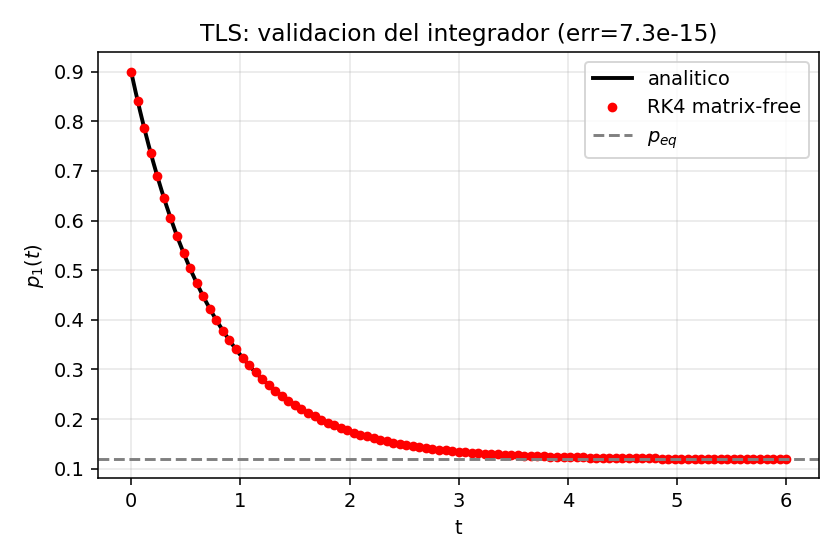
\includegraphics[width=\textwidth]{../figures/01_tls_validation.png}
\end{minipage}\hfill
\begin{minipage}{0.48\textwidth}\centering
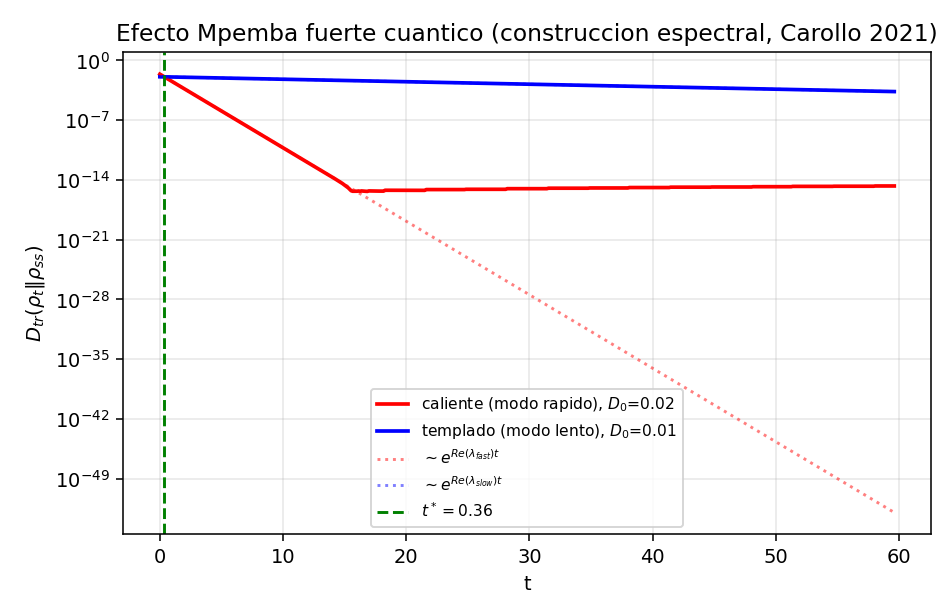
\includegraphics[width=\textwidth]{../figures/03_mpemba_strong.png}
\end{minipage}
\caption{Izquierda: validación del integrador \emph{matrix-free} en el TLS (RK4
sobre la solución exacta, error ${\sim}10^{-15}$). Derecha: \textbf{efecto Mpemba
fuerte} construido por geometría espectral en el sistema $\Lambda$ de tres
niveles ---la preparación que excita el modo rápido parte más lejos del
equilibrio (mayor $D_0$) pero lo alcanza antes, cruzando a la que excita el modo
lento en $t^*\approx0.36$. Las pendientes asintóticas siguen
$e^{\operatorname{Re}(\lambda)t}$ de los modos respectivos.}
\label{fig:validacion}
\end{figure}

\subsection{Núcleo HPC: ejecución y escalado}

El núcleo en C++ se compila con la cadena del proyecto (OpenMPI${+}$GCC) y se
ejecuta distribuyendo las preparaciones entre rangos:
\begin{verbatim}
cd cpp && mkdir build && cd build
cmake .. -DMPI_CXX_COMPILER=/usr/bin/mpicxx.openmpi
make
OMP_NUM_THREADS=4 mpirun.openmpi --oversubscribe -np 2 ./qmpe_hpc ../config.ini
python ../../python/plot_hpc.py results
\end{verbatim}
Para la cadena de Ising disipativa de $N=4$ espines ($d=16$, $\dim\mathbb L=256^2$)
con seis preparaciones repartidas en 2 rangos${\times}$4 hilos, la evolución
completa hasta $t_{\max}=8$ con $\Delta t=2\times10^{-3}$ tarda ${\approx}6$~s y el
análisis posterior detecta los cruces de las curvas $D_{HS}(t)$
(Figura~\ref{fig:hpc}). Este es el punto de partida sobre el que aplicar las costuras
de paralelización de la Sección~8: almacenamiento disperso, trayectorias en MPI y
modos lentos con SLEPc.

\begin{figure}[h]
\centering
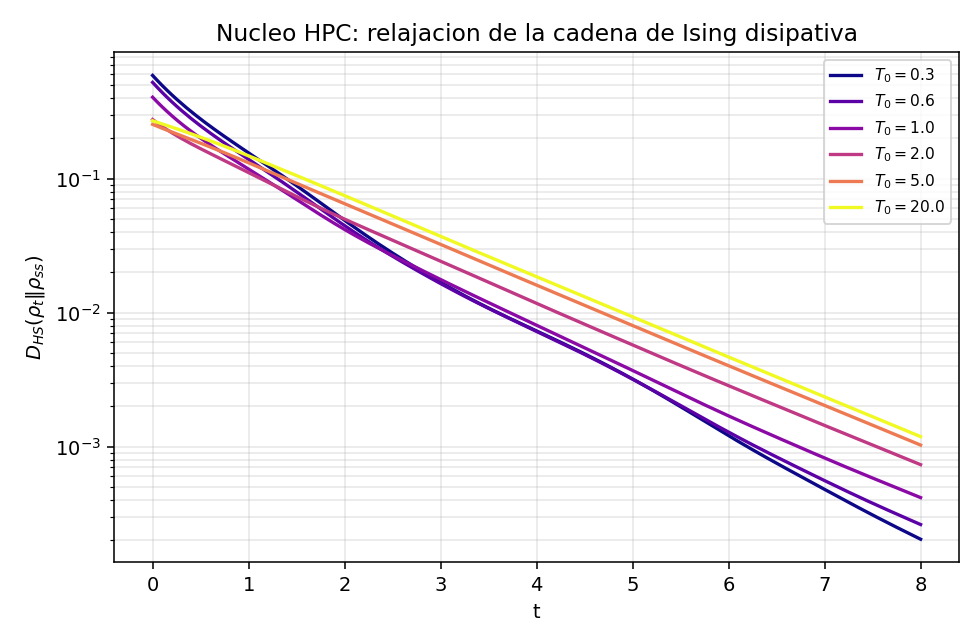
\includegraphics[width=0.72\textwidth]{../figures/qmpe_hpc_curves.png}
\caption{Salida del núcleo HPC: relajación $D_{HS}(\rho_t\|\rho_{ss})$ de la
cadena de Ising disipativa ($N=4$) para distintas preparaciones $T_0$, calculada
con el integrador \emph{matrix-free} paralelo. El cruce de curvas es la firma del
efecto; su interpretación (directo/inverso) depende de $T_0$ frente a
$T_{\rm bath}$.}
\label{fig:hpc}
\end{figure}

\subsection{Estado de las costuras de paralelización}

La implementación distingue lo \emph{ya paralelizado} de lo \emph{preparado para
paralelizar}, marcado en el código con \texttt{// [PARALELIZAR]}:

\begin{itemize}[leftmargin=1.6em,itemsep=2pt]
\item[\checkmark] \textbf{OpenMP intranodo} sobre el producto de matrices del SpMV.
\item[\checkmark] \textbf{MPI internodo} sobre el barrido de preparaciones/parámetros.
\item[$\circ$] \textbf{Matrix-free disperso} (CSR de $H,L_\mu$) para $N\gtrsim8$.
\item[$\circ$] \textbf{Trayectorias cuánticas en MPI} (T3a, escala casi perfecta).
\item[$\circ$] \textbf{Modos lentos con SLEPc/PETSc} (T1, \emph{shift-invert} $\sigma{=}0$).
\item[$\circ$] \textbf{GPU} (cuSPARSE / redes tensoriales) para muchos cuerpos (T3b).
\end{itemize}

%====================================================================
\section{Conclusiones y direcciones}
%====================================================================

El efecto Mpemba cuántico es, en su núcleo, un fenómeno de \emph{geometría espectral} de un generador no
normal: la relajación anómala surge cuando el estado inicial evita los modos lentos del Liouvilliano
\cite{Carollo2021,LiYang2026,AresCalabreseMurciano2025}. Esta lectura tiene una virtud práctica decisiva
para HPC: todas las cantidades de interés —tasas $\lambda_k$, modos $\hat r_k,\hat l_k$, solapamientos
$a_k$, distancias $\Dop(\rho_t\|\rss)$ y QFI $F_T$— se reducen a tres primitivas numéricas (SpMV, problema de
autovalores interior, acción del exponencial de matriz) que están bien soportadas por bibliotecas paralelas
maduras (PETSc/SLEPc, Expokit) y, en muchos cuerpos, por trayectorias cuánticas (paralelas) y redes
tensoriales.

La hoja de ruta para tener dominio cuantitativo del fenómeno es: (1)~validar el núcleo con modelos resolubles
(TLS, Dicke); (2)~implementar el diagnóstico espectral y de distancias en pocos cuerpos con SLEPc;
(3)~escalar a muchos cuerpos con trayectorias y/o redes tensoriales; (4)~explotar el efecto, computando la
rotación óptima de aceleración \cite{Carollo2021,Kochsiek2022} y mapeando la ganancia metrológica de QFI
\cite{Chattopadhyay2026,LiYang2026}. Direcciones abiertas de alto valor incluyen el régimen no markoviano
\cite{Strachan2025}, los puntos excepcionales y la dinámica oscilatoria \cite{Chatterjee2024}, y la
caracterización de recurso de las correlaciones cuánticas que amplían la ventana de Mpemba
\cite{Alyuruk2025,Summer2026}.

\bigskip
\noindent\textit{Nota de alcance.} Este informe sintetiza el marco teórico y numérico a partir de la
literatura del proyecto. Las afirmaciones técnicas concretas (formas de los generadores, criterios
espectrales, resultados experimentales) están referenciadas; los detalles de rendimiento dependerán de la
plataforma de HPC concreta y deben medirse empíricamente en la fase de implementación.

\bibliographystyle{unsrt}
\bibliography{referencias}

\end{document}
